\subsection{Speedup with varying matrix size}
In this subsection, the speedup of the \texttt{omp3} parallelization is investigated with changing matrix sizes. The threshold level is chosen individually for each size such that the program runs for at least a few seconds. The resulting curves can be seen in figure \ref{fig:speedup_N}. Despite the differing thresholds, the curves are still comparable due to the fact that the parallel region is outside the loop in \texttt{omp3}, which means that each iteration is identical, and so a larger number of iterations does not influence the speedup because it is relative to the case with one processor. The number of iterations for a single curve is constant for all number of processors. For a small number of processors, the speedup is similar, but as the number of processors increase, so does the parallel overhead required to keep track of the threads. This limits the speedup, and for a large number of processors, it even decreases for matrix sizes of $N = 500$ and $N = 1000$. For $N = 100$ the quickest is to use one core, simply because the overhead of even two cores takes more time than is gained by the parallelization. For $N = 10000$ the speedup is not seen to decrease because the matrix is so large that the speed gained from the parallelization is larger than the loss from the parallel overhead. If a larger number of cores was available, a decrease in speedup is expected. For $N = 100$, the analyzer tool was used to confirm our hypothesis: For 1 core, the program took $\sim 2.5$ s to run, but for 10 cores, the program spent 39 s on the implicit barriers after the for loops alone, i.e. a lot of work is done to keep track of the synchronization of the threads while the fraction of time where they are actually working is very small. And that is even when the parallel region is outside the main while loop, so the worker team is not destroyed on each iteration, but it is put to sleep and woken up many times, which also affect performance.

\subsection{Speedup with different compiler option}

\begin{figure}
\centering
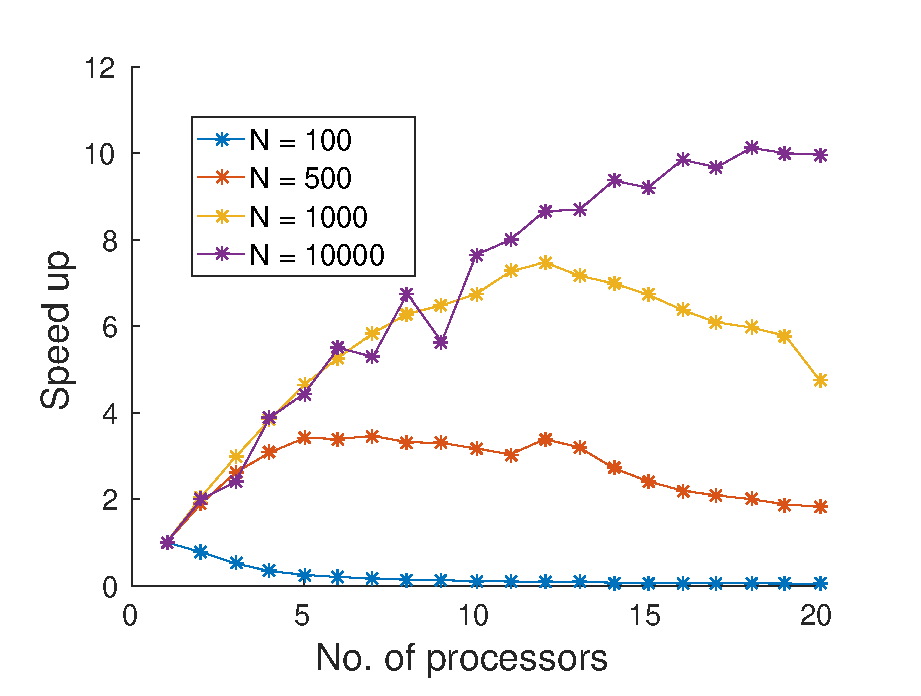
\includegraphics[width = 0.8\textwidth]{fig/speedup_N.eps}
\caption{The speedup of the Jacobi iteration with the best parallellization method, \texttt{omp3}, with different matrix sizes.}
\label{fig:speedup_N}
\end{figure}
